\makeatletter \def\NR@nopatch@beamer{} \makeatother %Temporary due to bug on 17 May

\documentclass{beamer}\usepackage[]{graphicx}\usepackage[]{xcolor}
% maxwidth is the original width if it is less than linewidth
% otherwise use linewidth (to make sure the graphics do not exceed the margin)
\makeatletter
\def\maxwidth{ %
  \ifdim\Gin@nat@width>\linewidth
    \linewidth
  \else
    \Gin@nat@width
  \fi
}
\makeatother

\definecolor{fgcolor}{rgb}{0.345, 0.345, 0.345}
\newcommand{\hlnum}[1]{\textcolor[rgb]{0.686,0.059,0.569}{#1}}%
\newcommand{\hlstr}[1]{\textcolor[rgb]{0.192,0.494,0.8}{#1}}%
\newcommand{\hlcom}[1]{\textcolor[rgb]{0.678,0.584,0.686}{\textit{#1}}}%
\newcommand{\hlopt}[1]{\textcolor[rgb]{0,0,0}{#1}}%
\newcommand{\hlstd}[1]{\textcolor[rgb]{0.345,0.345,0.345}{#1}}%
\newcommand{\hlkwa}[1]{\textcolor[rgb]{0.161,0.373,0.58}{\textbf{#1}}}%
\newcommand{\hlkwb}[1]{\textcolor[rgb]{0.69,0.353,0.396}{#1}}%
\newcommand{\hlkwc}[1]{\textcolor[rgb]{0.333,0.667,0.333}{#1}}%
\newcommand{\hlkwd}[1]{\textcolor[rgb]{0.737,0.353,0.396}{\textbf{#1}}}%
\let\hlipl\hlkwb

\usepackage{framed}
\makeatletter
\newenvironment{kframe}{%
 \def\at@end@of@kframe{}%
 \ifinner\ifhmode%
  \def\at@end@of@kframe{\end{minipage}}%
  \begin{minipage}{\columnwidth}%
 \fi\fi%
 \def\FrameCommand##1{\hskip\@totalleftmargin \hskip-\fboxsep
 \colorbox{shadecolor}{##1}\hskip-\fboxsep
     % There is no \\@totalrightmargin, so:
     \hskip-\linewidth \hskip-\@totalleftmargin \hskip\columnwidth}%
 \MakeFramed {\advance\hsize-\width
   \@totalleftmargin\z@ \linewidth\hsize
   \@setminipage}}%
 {\par\unskip\endMakeFramed%
 \at@end@of@kframe}
\makeatother

\definecolor{shadecolor}{rgb}{.97, .97, .97}
\definecolor{messagecolor}{rgb}{0, 0, 0}
\definecolor{warningcolor}{rgb}{1, 0, 1}
\definecolor{errorcolor}{rgb}{1, 0, 0}
\newenvironment{knitrout}{}{} % an empty environment to be redefined in TeX

\usepackage{alltt}
\usepackage{graphicx}
\usepackage{graphicx}
\usepackage{verbatim}
\usepackage{etoolbox}
\usepackage{everysel}
% \usepackage{enumitem}

%% This package allows text highlighting
\usepackage{soul}

%% This sets the theme of the presentation which controls
%% the formatting of the slides
\usetheme{Boadilla}

%% Turn off the navigation symbols
\setbeamertemplate{navigation symbols}{} 

%% Change the default itemize [ball]s to [circle]s
\setbeamertemplate{itemize items}[circle]

%% Change the default enumerate [ball]s to plain text
\setbeamertemplate{enumerate items}[default]

%% Load the enumitem package and ensure it works nicely with beamer
% \setitemize{label=\usebeamerfont*{itemize item}
%   \usebeamercolor[fg]{itemize item}
%   \usebeamertemplate{itemize item}}
% \setenumerate{label=\usebeamerfont*{enumerate item}
%   \usebeamercolor[fg]{enumerate item}
%   \usebeamertemplate{enumerate item}}

%% Set the author block so STATS 201/8 appears on every
\author{STATS 201/8}

%% Clear the date block
\date{}


\setbeamercolor{title}{bg=blue!40}
\setbeamerfont{title}{size=\LARGE,series=\bfseries}

%%Sectioning commands
\setbeamercolor{section title}{bg=blue!20}
\setbeamerfont{section title}{size=\large}

\setbeamertemplate{section page}{%
    \begingroup
        \begin{beamercolorbox}[sep=10pt,center,rounded=true,shadow=true]{section title}
        \usebeamerfont{section title}Section~\thechapter.\thesection \newline \insertsection\par
        \end{beamercolorbox}
		\vfill
    \endgroup
}

\newcommand{\BeginSection}[1]{\section{#1} \frame{\sectionpage}}
%\AtBeginSection[]{%
%    \begin{frame}
%        \sectionpage
%    \end{frame}
%}


%% This makes all equations blue
\AtBeginEnvironment{equation*}{\color{blue}}
\AtBeginEnvironment{align*}{\color{blue}}
\everymath{\color{blue}}

%% This puts a 0 point space between paragraphs, means we don't need to use vspace, or list environments if 
%% we don't want to
\setlength{\parskip}{0pt}


%% Russell: removes spaces after R input/output?
\setlength{\topsep}{0.5mm}

%% David: In addition to Russel's command to remove spaces after R input/output, these commands remove the space between R input/output.
%% Stackoverflow link: https://stackoverflow.com/questions/35734525/reduce-space-between-code-chunks-and-code-output-in-rmarkdown-beamer-presentatio
%% \setlength{\OuterFrameSep}{-2pt}
\makeatletter
\preto{\@verbatim}{\topsep=-1pt \partopsep=-1pt }
\makeatother

%% Some useful colors
\definecolor{darkgreen}{rgb}{0.176,0.486,0.031}
\definecolor{redbrown}{HTML}{950605}
\definecolor{darkred}{HTML}{d80605}


%% nice little macro for changing the font of R code
\newcommand{\rcode}[1]{\protect{\color{darkgreen}\texttt{#1}}}

%% macro for bold blue italics
\newcommand{\blueBoldEmph}[1]{{\color{blue}\textbf{\emph{#1}}}}

% ~iid macro
\newcommand{\iid }{\stackrel{iid}{\sim}}

%% Macro for t-test amd P-value
\newcommand{\ttest}{\emph{t}-test}
\newcommand{\pval}{\emph{P}-value}

%% Statistics operators 
\DeclareMathOperator{\Bias}{Bias}
\DeclareMathOperator{\Cov}{Cov}
\DeclareMathOperator*{\Cor}{Cor}
\DeclareMathOperator{\E}{E}
\DeclareMathOperator{\MSE}{MSE}
\DeclareMathOperator{\Odds}{Odds}
\DeclareMathOperator{\OR}{OR}
\DeclareMathOperator{\PMSE}{PMSE}
\DeclareMathOperator{\sd}{sd}
\DeclareMathOperator{\se}{se}
\DeclareMathOperator*{\Var}{Var}
\DeclareMathOperator{\logit}{logit}

%% Should see if can make this a mathop
\newcommand{\comb}[2]{\mbox{$\big(_{#2}^{#1}\big)$}}




%\DeclareMathOperator{\E}{{E}}
%\DeclareMathOperator{\Var}{{Var}}
%\DeclareMathOperator{\sd}{{sd}}
%\DeclareMathOperator{\se}{{se}}
%\newcommand{\comb}[2]{\mbox{$\big(_{#2}^{#1}\big)$}}
%\DeclareMathOperator{\Odds}{{Odds}}
%\DeclareMathOperator{\OR}{{OR}}
% \newcommand{\vs}{\vspace{2mm}}

% \setlength{\parskip}{7pt}
% \setlength{\topsep}{0mm} %To reduce line spacing in R output
\IfFileExists{upquote.sty}{\usepackage{upquote}}{}
\begin{document}
\newcommand{\thechapter}{13}
\title{Chapter \thechapter: \\ Modelling count data using the Poisson distribution}
\institute{University of Auckland}




\begin{frame}
\titlepage
\end{frame}


\begin{frame}[t]
\frametitle{Learning Outcomes}
In this chapter you will learn about:
\begin{center}
\vspace{16pt}
\begin{minipage}{0.9\textwidth}
  \begin{itemize}
  \item The nature of count data
  \item Example - modelling the number of R packages
  \item The Poisson Distribution
  \item The generalized linear model (GLM)
  \item GLM re-analysis of the example
  \item The quasi-Poisson correction
  \item Interpretting the fitted GLM
  \item Relevant \rcode{R}-code.
  \end{itemize}
\end{minipage}
\end{center}

\end{frame}


%%%%%%%%%%%%%%%%%%%%%%%%%%%%%%%%%%%%%%%%%%%%%%%%%%%%%%%%%%%%%%%%%%%%%%%%%%%%%%%%%%%%%%%%%%%
\BeginSection{The nature of count data}
%%%%%%%%%%%%%%%%%%%%%%%%%%%%%%%%%%%%%%%%%%%%%%%%%%%%%%%%%%%%%%%%%%%%%%%%%%%%%%%%%%%%%%%%%%%



\begin{frame}[fragile]
\frametitle{The nature of count data}
In many studies the {\bf response} variable will be a count.
\bigskip

A count variable is one where the measurement is the count of the number of times
some event occurs.
Obviously, it can only take values that belong to the non-negative integers
\{0,1,2,3...\}.
\bigskip

In statistical parlance, a count variable is an example of a {\em discrete} variable,
since the values it can take are discretely separated.
\bigskip

(In contrast,
a variable with a Normal Distribution is an example of a {\em continuous variable},
since if can take any value on a continuum.)
\end{frame}



\begin{frame}[fragile]
\frametitle{The nature of count data\ldots}
In this course we shall encounter three types of count data:
\bigskip

\begin{enumerate}
  \item Counts of the number of ``events'' occurring, where ideally, the events occur independently of one another and with no specific upper limit on the maximum number.
  \item Counts of the number of ``successes''\footnote{Here, ``successes'' is used generically. E.g., It could be the number of females in a class of 146.} from a fixed number of trials. E.g., the number of Heads from tossing a coin 10 times. In this case, the response variable $y$ is the proportion of successes (see Chapter 15).
  \item Counts of the number of items in a category. E.g., The count of A, B, and C grades in the course.
\end{enumerate}
\bigskip

In this Chapter we focus on the first of the above types. Some examples are given below.
\end{frame}



\begin{frame}[fragile]
\frametitle{The nature of count data\ldots}
\framesubtitle{Some examples of counting the number of events occurring}
\begin{itemize}
\item The success of a marketing campaign can be assessed by analysing the change in
number of purchases.
\item In epidemiology, the spread of an infectious disease can be modelled by observing
the number of those infected each day.
\item In operations research, a business can run more efficiently by being able to predict the number of customer interactions in a day,
and hence the number of staff required.
\item In ecology, the success of habitat restoration can be assessed by gathering counts
of the number of animals before and after the restoration.
\item The efficacy of fluoridation can be assessed by counting the number of tooth cavities
in the mouths of subjects.
\end{itemize}
\bigskip

{\bf Question:} For which of the above scenarios would it be reasonable to assume that the events being counted are occurring independently?
\end{frame}


\begin{frame}[fragile]
\frametitle{Analysis of count data}
\framesubtitle{Why do we care?}

In some situations linear regression can be successfully used to analyse count data. In fact, you may have already seen this done in this course. However, these are special cases.\footnote{We will soon see an example where an inappropriate application of a linear regression model to count data was responsible for the most expensive human mistake in history (up to that point in time).}
\bigskip \bigskip

{\bf Linear regression is not generally applicable to count data.} This is demonstrated in the example below.
\end{frame}


%%%%%%%%%%%%%%%%%%%%%%%%%%%%%%%%%%%%%%%%%%%%%%%%%%%%%%%%%%%%%%%%%%%%%%%%%%%%%%%%%%%%%%%%%%%
\BeginSection{Example: Number of R packages submitted to the \\ Comprehensive R Archive Network (CRAN)}
%%%%%%%%%%%%%%%%%%%%%%%%%%%%%%%%%%%%%%%%%%%%%%%%%%%%%%%%%%%%%%%%%%%%%%%%%%%%%%%%%%%%%%%%%%%



\begin{frame}[fragile]
\frametitle{Submissions to CRAN}
In the following example we will model a count variable (number of R packages submitted to the CRAN over the years) using what we know to date: the {\em linear model} via the function \rcode{lm}. 
\bigskip

We will contrast this to a more general and more appropriate way of modelling counts: the {\em generalized linear model} (GLM) via the function \rcode{glm}.
\bigskip

Along the way you will be introduced to a new distribution, the Poisson distribution.

\end{frame}


\begin{frame}[fragile]
\frametitle{Submissions to CRAN\ldots}

As \rcode{R} is an open-source programming environment, people are encouraged to submit software packages used in their research for others to access via the CRAN\footnote{You probably downloaded your R installation from the CRAN.}, which was created in 2005. We would like to understand the nature of its growth. With this in mind, the number of new packages submitted in each year, from 2005 to 2016, has been recorded:

% note well - original CRAN submissons data now called in CRANold.txt has changed dramatically - hence  CRAN.txt (new & revised)
\begin{knitrout}\scriptsize
\definecolor{shadecolor}{rgb}{0.969, 0.969, 0.969}\color{fgcolor}\begin{kframe}
\begin{alltt}
\hlstd{> }\hlstd{CRAN.df} \hlkwb{=} \hlkwd{read.table}\hlstd{(}\hlstr{"Data/CRAN.txt"}\hlstd{,} \hlkwc{header}\hlstd{=T)}
\hlstd{> }\hlstd{CRAN.df}
\end{alltt}
\begin{verbatim}
   Year Number
1  2005      1
2  2006      4
3  2007      2
4  2008     10
5  2009     32
6  2010     44
7  2011     89
8  2012    594
9  2013    830
10 2014   1185
11 2015   1944
12 2016   4512
\end{verbatim}
\end{kframe}
\end{knitrout}

\end{frame}


\begin{frame}[fragile]
\frametitle{Submissions to CRAN\ldots}
\framesubtitle{Plotting the data}

\begin{knitrout}\scriptsize
\definecolor{shadecolor}{rgb}{0.969, 0.969, 0.969}\color{fgcolor}\begin{kframe}
\begin{alltt}
\hlstd{> }\hlcom{## One-by-two figure layout}
\hlstd{> }\hlkwd{par}\hlstd{(}\hlkwc{mfrow}\hlstd{=}\hlkwd{c}\hlstd{(}\hlnum{1}\hlstd{,}\hlnum{2}\hlstd{))}
\hlstd{> }\hlcom{## Scatter plot using raw y}
\hlstd{> }\hlkwd{plot}\hlstd{(Number} \hlopt{~} \hlstd{Year,} \hlkwc{data} \hlstd{= CRAN.df)}
\hlstd{> }\hlcom{## Scatter plot using log y}
\hlstd{> }\hlkwd{plot}\hlstd{(}\hlkwd{log}\hlstd{(Number)} \hlopt{~} \hlstd{Year,} \hlkwc{data} \hlstd{= CRAN.df)}
\end{alltt}
\end{kframe}
\end{knitrout}



\begin{figure}
   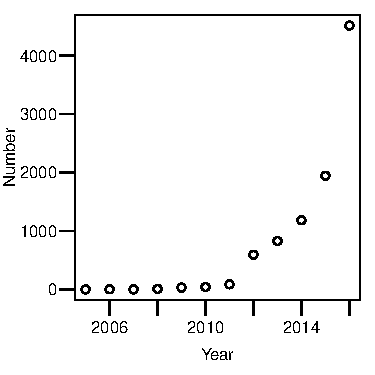
\includegraphics[width=0.475\textwidth]{figure/RC-H13-003A}
   \hfill
   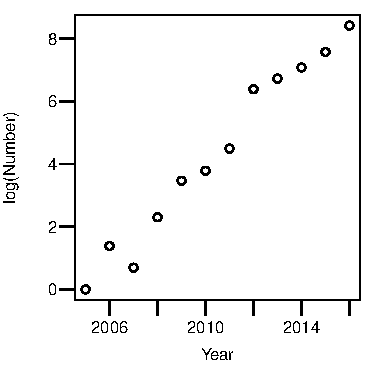
\includegraphics[width=0.475\textwidth]{figure/RC-H13-003B}
\end{figure}

\end{frame}


\begin{frame}[fragile]
\frametitle{Submissions to CRAN\ldots}
\framesubtitle{Analysis via \rcode{lm}}
\label{pg:CRAN LM}
The relationship between year and number of submissions looks reasonably linear on the log scale, so we'll fit a linear model to $\log(Y)$.
\medskip

\begin{knitrout}\scriptsize
\definecolor{shadecolor}{rgb}{0.969, 0.969, 0.969}\color{fgcolor}\begin{kframe}
\begin{alltt}
\hlstd{> }\hlstd{CRAN.fit} \hlkwb{=} \hlkwd{lm}\hlstd{(}\hlkwd{log}\hlstd{(Number)} \hlopt{~} \hlstd{Year,} \hlkwc{data} \hlstd{= CRAN.df)}
\hlstd{> }\hlkwd{plot}\hlstd{(CRAN.fit,}\hlkwc{which}\hlstd{=}\hlnum{1}\hlstd{)}
\end{alltt}
\end{kframe}
\end{knitrout}



\begin{figure}
  \centering
  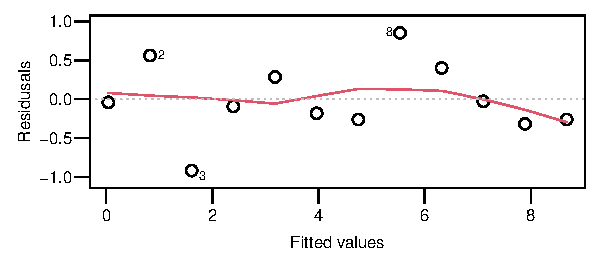
\includegraphics[scale = 0.9]{figure/RC-H13-005a}
\end{figure}

No concerns.
\end{frame}


\begin{frame}[fragile]
\frametitle{Submissions to CRAN\ldots}
\framesubtitle{Analysis via \rcode{lm}}
\label{pg:LMcooks20x}

\begin{knitrout}\scriptsize
\definecolor{shadecolor}{rgb}{0.969, 0.969, 0.969}\color{fgcolor}\begin{kframe}
\begin{alltt}
\hlstd{> }\hlkwd{cooks20x}\hlstd{(CRAN.fit)}
\end{alltt}
\end{kframe}
\end{knitrout}



\begin{figure}
  \centering
  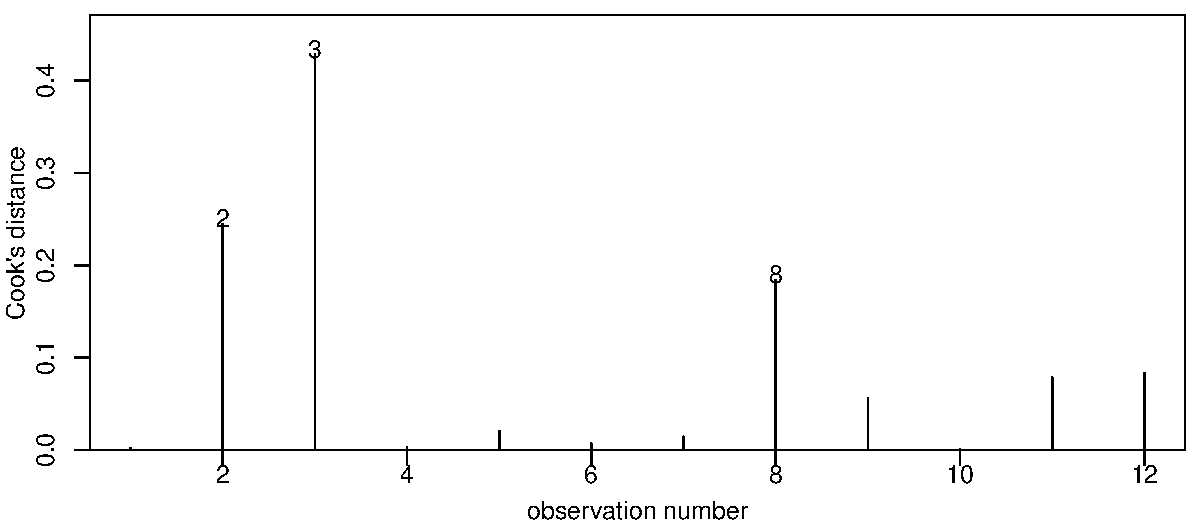
\includegraphics[scale = 0.5]{figure/RC-H13-005b}
\end{figure}

The Cook's distance for observation 3 exceeds our threshold of 0.4. However, with only 12 observations this is perhaps not of great concern.
\end{frame}



\begin{frame}[fragile]
\frametitle{Submissions to CRAN\ldots}
\framesubtitle{Analysis via \rcode{lm}\ldots}



\begin{figure}
  \centering
  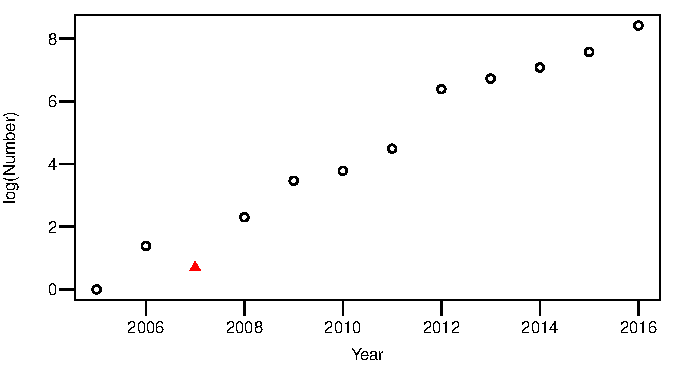
\includegraphics{figure/RC-H13-006}
\end{figure}

Indeed, the third observation in {\color{red}red} does not seem to be influential in the exploratory plots. So, we will keep it in the model.
\end{frame}



\begin{frame}[fragile]
\frametitle{Submissions to CRAN\ldots}
\framesubtitle{Analysis via \rcode{lm}\ldots}


\begin{knitrout}\scriptsize
\definecolor{shadecolor}{rgb}{0.969, 0.969, 0.969}\color{fgcolor}\begin{kframe}
\begin{alltt}
\hlstd{> }\hlkwd{summary}\hlstd{(CRAN.fit)}
\end{alltt}
\end{kframe}
\end{knitrout}

\begin{knitrout}\scriptsize
\definecolor{shadecolor}{rgb}{0.969, 0.969, 0.969}\color{fgcolor}\begin{kframe}
\begin{verbatim}
Coefficients:
              Estimate Std. Error t value Pr(>|t|)    
(Intercept) -1.574e+03  8.245e+01  -19.09 3.39e-09 ***
Year         7.849e-01  4.101e-02   19.14 3.30e-09 ***
---
Residual standard error: 0.4904 on 10 degrees of freedom
Multiple R-squared:  0.9734,	Adjusted R-squared:  0.9708 
F-statistic: 366.4 on 1 and 10 DF,  p-value: 3.295e-09
\end{verbatim}
\end{kframe}
\end{knitrout}

\end{frame}



\begin{frame}[fragile]
\frametitle{Submissions to CRAN\ldots}
\framesubtitle{Analysis via \rcode{lm}\ldots}
Back-transform to get the multiplicative effect of year.
\bigskip

\begin{knitrout}\scriptsize
\definecolor{shadecolor}{rgb}{0.969, 0.969, 0.969}\color{fgcolor}\begin{kframe}
\begin{alltt}
\hlstd{> }\hlcom{## Estimated annual multiplier}
\hlstd{> }\hlkwd{exp}\hlstd{(CRAN.fit}\hlopt{$}\hlstd{coef[}\hlstr{"Year"}\hlstd{])}
\end{alltt}
\begin{verbatim}
    Year 
2.192237 
\end{verbatim}
\begin{alltt}
\hlstd{> }\hlcom{## Confidence interval}
\hlstd{> }\hlkwd{exp}\hlstd{(}\hlkwd{confint}\hlstd{(CRAN.fit))}
\end{alltt}
\begin{verbatim}
              2.5 %  97.5 %
(Intercept) 0.00000 0.00000
Year        2.00081 2.40198
\end{verbatim}
\end{kframe}
\end{knitrout}

\bigskip

So, the Executive Summary would have said that the median annual number of submissions to CRAN multiplies by between 2.00 to 2.40 times each year.
In other words, it increases by between 100\% and 140\% per annum.
\end{frame}


\begin{frame}[fragile]
\frametitle{Submissions to CRAN\ldots}
\framesubtitle{Analysis via \rcode{lm}\ldots}

We will use this model to estimate the median of the distribution of the number of submissions in 2017.
\bigskip


\begin{knitrout}\scriptsize
\definecolor{shadecolor}{rgb}{0.969, 0.969, 0.969}\color{fgcolor}\begin{kframe}
\begin{alltt}
\hlstd{> }\hlstd{predCRAN.df} \hlkwb{=} \hlkwd{data.frame}\hlstd{(}\hlkwc{Year} \hlstd{=} \hlnum{2017}\hlstd{)}
\hlstd{> }\hlstd{pred2017} \hlkwb{=} \hlkwd{predict}\hlstd{(CRAN.fit, predCRAN.df,} \hlkwc{interval} \hlstd{=} \hlstr{"confidence"}\hlstd{)}
\hlstd{> }
\hlstd{> }\hlcom{## Prediction on the log scale}
\hlstd{> }\hlstd{pred2017}
\end{alltt}
\begin{verbatim}
      fit     lwr      upr
1 9.45978 8.78731 10.13225
\end{verbatim}
\begin{alltt}
\hlstd{> }\hlcom{## Back-transform for the median of the number of submissions in 2017}
\hlstd{> }\hlkwd{exp}\hlstd{(pred2017)}
\end{alltt}
\begin{verbatim}
       fit      lwr      upr
1 12833.05 6550.586 25140.85
\end{verbatim}
\end{kframe}
\end{knitrout}

\medskip

So, the Executive Summary would have said that the median of the number of submissions to CRAN in 2017 is between 6550 and 25100. 

\end{frame}


\begin{frame}[fragile]
\frametitle{Submissions to CRAN\ldots}
\framesubtitle{Comments on the analysis via \rcode{lm}\ldots}
There is a well known saying:
\medskip

``If you only have a hammer, you tend to see every problem as a nail." -- Abraham Maslow [Replace ``hammer" with ``linear model", and ``a nail" with ``normally distributed"]
\bigskip

We were able to do an analysis with \rcode{lm} (our hammer) by working with the logged data (our normally distributed nails). But, was this really a sensible way to analyse the CRAN data?
\bigskip

Before we answer this question, we'll look at a different methodology that is tailored for the analysis of count data. The first thing we need is a more appropriate type of distribution to replace the normal distribution. One that is tailored for describing the distribution of count data.
\end{frame}


%%%%%%%%%%%%%%%%%%%%%%%%%%%%%%%%%%%%%%%%%%%%%%%%%%%%%%%%%%%%%%%%%%%%%%%%%%%%%%%%%%%%%%%%%%%
\BeginSection{The Poisson Distribution}
%%%%%%%%%%%%%%%%%%%%%%%%%%%%%%%%%%%%%%%%%%%%%%%%%%%%%%%%%%%%%%%%%%%%%%%%%%%%%%%%%%%%%%%%%%%



\begin{frame}[fragile]
\frametitle{The Poisson distribution}
Statisticians often use the Poisson distribution to describe the behaviour of counts of events that occur randomly in space or time, such as:
\medskip

\begin{itemize}
\item The number of alcohol related arrivals at a hospital.

\item The number of dolphins in a pod.

\item The number of pods of dolphins sighted during an aerial survey.

\item The annual number of road fatalities.

\item The annual number of fatal road accidents.
\end{itemize}
\bigskip

The Poisson is a distribution that takes values on the non-negative integers
\{0,1,2,3,...\} and it has no upper limit.
\bigskip

The Poisson distribution is specified by a single parameter, its mean (i.e., expected value).
We will write, Pois($\mu$) to denote a Poisson distribution with mean of $\mu$.
\end{frame}



\begin{frame}[fragile]
\frametitle{The Poisson distribution\ldots}
The probability that the non-negative integer value $y$ will be observed if generated
by a Pois($\mu$) distribution is given by the following formula:
\[
\Pr(y)=\frac{\exp(-\mu)\mu^y}{y!} \ .
\]
where $y!=$ \rcode{factorial(y)} $=1 \times 2 \times ... \times (y-1) \times y$
(and $0!=1$).
\bigskip

For $y=12$ and $\mu=9.61$, this could be calculated in \rcode{R} using the code

\begin{knitrout}\scriptsize
\definecolor{shadecolor}{rgb}{0.969, 0.969, 0.969}\color{fgcolor}\begin{kframe}
\begin{alltt}
\hlstd{> }\hlstd{y}\hlkwb{=}\hlnum{12}\hlstd{; mu}\hlkwb{=}\hlnum{9.61}
\hlstd{> }\hlstd{(}\hlkwd{exp}\hlstd{(}\hlopt{-}\hlstd{mu)}\hlopt{*}\hlstd{mu}\hlopt{^}\hlstd{y)}\hlopt{/}\hlkwd{factorial}\hlstd{(y)}
\end{alltt}
\begin{verbatim}
[1] 0.08685078
\end{verbatim}
\end{kframe}
\end{knitrout}
\end{frame}



\begin{frame}[fragile]
\frametitle{The Poisson distribution\ldots}
In \rcode{R}, the in-built function \rcode{dpois}(y, $\mu$) calculates these Poisson probabilities.
E.g., the probability that $y=12$ will be observed from a Pois($9.61$) distribution is

\begin{knitrout}\scriptsize
\definecolor{shadecolor}{rgb}{0.969, 0.969, 0.969}\color{fgcolor}\begin{kframe}
\begin{alltt}
\hlstd{> }\hlkwd{dpois}\hlstd{(}\hlnum{12}\hlstd{,}\hlnum{9.61}\hlstd{)}
\end{alltt}
\begin{verbatim}
[1] 0.08685078
\end{verbatim}
\end{kframe}
\end{knitrout}
\bigskip

You can also generate random Poisson values. E.g., here are 20 random values from a Pois($10$)
distribution,
\begin{knitrout}\scriptsize
\definecolor{shadecolor}{rgb}{0.969, 0.969, 0.969}\color{fgcolor}\begin{kframe}
\begin{alltt}
\hlstd{> }\hlkwd{rpois}\hlstd{(}\hlnum{20}\hlstd{,}\hlnum{10}\hlstd{)}
\end{alltt}
\begin{verbatim}
 [1]  9  9  8 11 11  9 15  8 11 12 10  9 16  9  6  8 16 12  7 15
\end{verbatim}
\end{kframe}
\end{knitrout}

\end{frame}


\begin{frame}[fragile]
\frametitle{The Poisson distribution\ldots}
\framesubtitle{An example}
Suppose that a hospital {\em expects} to handle 3 victims of alcohol related mis-adventure
on a Friday night.
\bigskip

Assuming that the {\em actual} number on any given Friday night can be described by a Poisson distribution with
a mean of 3 (Pois($3$)), what does the distribution of the number of alchohol victims look like?
\end{frame}


\begin{frame}[fragile]
\frametitle{The Poisson distribution\ldots}
\framesubtitle{An example\ldots}
\begin{knitrout}\scriptsize
\definecolor{shadecolor}{rgb}{0.969, 0.969, 0.969}\color{fgcolor}\begin{kframe}
\begin{alltt}
\hlstd{> }\hlkwd{barplot}\hlstd{(}\hlkwd{dpois}\hlstd{(}\hlnum{0}\hlopt{:}\hlnum{12}\hlstd{,}\hlnum{3}\hlstd{),}\hlkwc{names}\hlstd{=}\hlnum{0}\hlopt{:}\hlnum{12}\hlstd{)}
\end{alltt}
\end{kframe}
\end{knitrout}



\begin{figure}
  \centering
  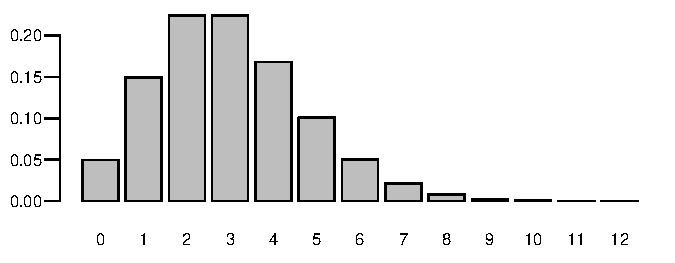
\includegraphics{figure/RC-H13-015}
\end{figure}

% Here are the actual probabilities, calculated for number of victims from 0 to 20,
% and printed to 6 decimal places accuracy:

\medskip

The probabilities for the number of victims from 0 to 20 are:
\begin{knitrout}\scriptsize
\definecolor{shadecolor}{rgb}{0.969, 0.969, 0.969}\color{fgcolor}\begin{kframe}
\begin{alltt}
\hlstd{> }\hlkwd{round}\hlstd{(}\hlkwd{dpois}\hlstd{(}\hlnum{0}\hlopt{:}\hlnum{20}\hlstd{,}\hlnum{3}\hlstd{),}\hlnum{6}\hlstd{)}
\end{alltt}
\begin{verbatim}
 [1] 0.049787 0.149361 0.224042 0.224042 0.168031 0.100819 0.050409 0.021604
 [9] 0.008102 0.002701 0.000810 0.000221 0.000055 0.000013 0.000003 0.000001
[17] 0.000000 0.000000 0.000000 0.000000 0.000000
\end{verbatim}
\end{kframe}
\end{knitrout}
\end{frame}


\begin{frame}[fragile]
\frametitle{The Poisson distribution\ldots}
\framesubtitle{More Poisson distributions}

% Plots of the Pois($10$) and Pois($100$) distributions:
\begin{knitrout}\scriptsize
\definecolor{shadecolor}{rgb}{0.969, 0.969, 0.969}\color{fgcolor}\begin{kframe}
\begin{alltt}
\hlstd{> }\hlkwd{par}\hlstd{(}\hlkwc{mfrow}\hlstd{=}\hlkwd{c}\hlstd{(}\hlnum{2}\hlstd{,}\hlnum{1}\hlstd{))} \hlcom{## Two-by-One figure layout}
\hlstd{> }\hlkwd{barplot}\hlstd{(}\hlkwd{dpois}\hlstd{(}\hlnum{0}\hlopt{:}\hlnum{25}\hlstd{,}\hlnum{10}\hlstd{),}\hlkwc{names}\hlstd{=}\hlnum{0}\hlopt{:}\hlnum{25}\hlstd{)} \hlcom{## Pois(10)}
\hlstd{> }\hlkwd{barplot}\hlstd{(}\hlkwd{dpois}\hlstd{(}\hlnum{50}\hlopt{:}\hlnum{150}\hlstd{,}\hlnum{100}\hlstd{),}\hlkwc{names}\hlstd{=}\hlnum{50}\hlopt{:}\hlnum{150}\hlstd{,}\hlkwc{las}\hlstd{=}\hlnum{1}\hlstd{)} \hlcom{## Pois(100)}
\end{alltt}
\end{kframe}
\end{knitrout}



\begin{figure}
  \centering
  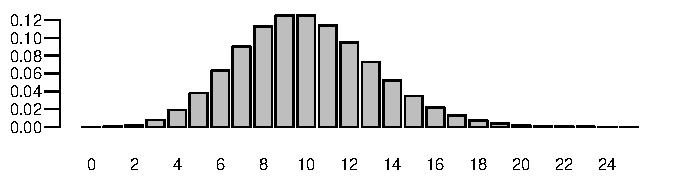
\includegraphics{figure/RC-H13-018A}
\end{figure}

\begin{figure}
  \centering
  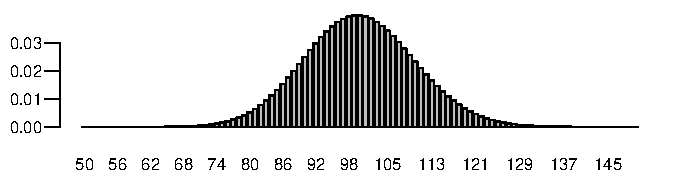
\includegraphics{figure/RC-H13-018B}
\end{figure}

\end{frame}


\begin{frame}
\frametitle{The Poisson distribution\ldots}
\framesubtitle{Properties of the Poisson distribution}
\begin{itemize}
\item Variability increases with the mean $\mu$.
In fact, the variance of a Pois($\mu$) is also $\mu$.
That is, if $Y$ is Pois($\mu$) distributed then
\[\Var(Y) = \E(Y) = \mu\]

\vspace{-1.5em}

\item The Poisson distribution is right-skewed for small values of $\mu$,
but looks very much like a (discretised) normal distribution for large $\mu$.
\end{itemize}
\end{frame}

\begin{frame}
\frametitle{The Poisson distribution\ldots}
\framesubtitle{Properties of the Poisson distribution\ldots}
The Poisson distribution is a good distribution to describe count data provided
that the events being counted are independent.
\begin{itemize}
\item The number of alcohol related arrivals at a hospital could be described by a Poisson distribution provided that the arrivals occur independently...does this seem reasonable to you???

\item What about the number of dolphins in a pod?

\item What about the number of pods of dolphins sighted during an aerial survey?

\item What about annual number of road fatalities?

\item What about annual number of fatal road accidents?
\end{itemize}

\bigskip


\begin{itemize}
\item Would it be sensible for an insurance company to assume that the number of earthquake damage claims was Poisson distributed?
\end{itemize}

\end{frame}



%%%%%%%%%%%%%%%%%%%%%%%%%%%%%%%%%%%%%%%%%%%%%%%%%%%%%%%%%%%%%%%%%%%%%%%%%%%%%%%%%%%%%%%%%%%
\BeginSection{The generalized linear model (GLM)}
%%%%%%%%%%%%%%%%%%%%%%%%%%%%%%%%%%%%%%%%%%%%%%%%%%%%%%%%%%%%%%%%%%%%%%%%%%%%%%%%%%%%%%%%%%%



\begin{frame}[fragile]
\frametitle{The generalized linear model}
Count data are not normally distributed, so we need to use a model that replaces the normality assumption with something more reasonable, such as assuming the data are Poisson distributed.
\bigskip

We will use a class of models called generalized linear models. They generalize the standard linear model (for normal data) by making it applicable to other types of data.
\bigskip

The linear model of Chaps 1-12 is a special case of a GLM.
\end{frame}



\begin{frame}[fragile]
\frametitle{The Poisson regression GLM for the CRAN data}
We will redo this analysis using a \rcode{GLM}. That is, the model will now assume that the number of packages in a given year is a Poisson random variable:
\vspace{-0.5em}
\[ Y \sim \text{Poisson}(\mu) \]
\vspace{-1.5em}

where the Poisson parameter ($\mu=E[Y]$) changes with respect to an $x$ variable as follows:
\vspace{-1.5em}

\[ \mu = \exp(\beta_0 + \beta_1 x). \]
\vspace{-1.5em}

Here, $x$ is year and $Y$ is the number of CRAN submissions in that year.
\medskip 

Since $\beta_0$ and $\beta_1$ can be negative or positive then so can $\beta_0 + \beta_1 x$, but $\mu = \exp(\beta_0 + \beta_1 x) > 0$, as required.
\medskip

The relationship $\mu = \exp(\beta_0 + \beta_1 x)$ can equivalently be expressed as 
\[\log(\mu) = \log E[Y|x] = \beta_0 + \beta_1 x \] 
and so sometimes people call this log-linear modelling.
\end{frame}



\begin{frame}[fragile]
\frametitle{Fitting a generalized linear model in \rcode{R}}
\framesubtitle{\rcode{glm} function}
Fitting a generalized linear model is the easy part. 
We simply use the \rcode{glm} function instead of \rcode{lm}, 
and instruct \rcode{glm} that the response variable is Poisson distributed by
giving it the \rcode{family = poisson} argument.

\medskip \medskip
{\bf NOTE:} Although only a simple change to the \rcode{R} code is required,
the methodology ``under the hood'' is very different.
It is no longer based on sums of squares,
and instead uses a technique called maximum likelihood.
\bigskip

Maximum likelihood is the most widely used tool in statistical estimation.
Linear regression (of normally distributed data) is a special case of 
maximum likelihood. 

\medskip 
For more on maximum likelihood, see STATS 310, 330 and 730.
\end{frame}





\begin{frame}[fragile]
\frametitle{Submissions to CRAN using Poisson regression}
\framesubtitle{Analysis via \rcode{glm}}
\begin{knitrout}\scriptsize
\definecolor{shadecolor}{rgb}{0.969, 0.969, 0.969}\color{fgcolor}\begin{kframe}
\begin{alltt}
\hlstd{> }\hlstd{CRAN.gfit} \hlkwb{=} \hlkwd{glm}\hlstd{(Number} \hlopt{~} \hlstd{Year,} \hlkwc{family} \hlstd{= poisson,} \hlkwc{data} \hlstd{= CRAN.df)}
\hlstd{> }\hlkwd{summary}\hlstd{(CRAN.gfit)}
\end{alltt}
\end{kframe}
\end{knitrout}

\begin{knitrout}\scriptsize
\definecolor{shadecolor}{rgb}{0.969, 0.969, 0.969}\color{fgcolor}\begin{kframe}
\begin{verbatim}
Call:
glm(formula = Number ~ Year, family = poisson, data = CRAN.df)

Coefficients:
              Estimate Std. Error z value Pr(>|z|)    
(Intercept) -1.282e+03  1.384e+01  -92.64   <2e-16 ***
Year         6.401e-01  6.868e-03   93.20   <2e-16 ***
---
(Dispersion parameter for poisson family taken to be 1)

    Null deviance: 19374.51  on 11  degrees of freedom
Residual deviance:   402.61  on 10  degrees of freedom
\end{verbatim}
\end{kframe}
\end{knitrout}

\end{frame}


\begin{frame}[fragile]
% \frametitle{Submissions to CRAN via  --  \rcode{glm}}
\frametitle{Submissions to CRAN using Poisson regression\ldots}
\framesubtitle{Assumption checks}

\smallskip

First, check the residuals to see if they look random.

\begin{knitrout}\scriptsize
\definecolor{shadecolor}{rgb}{0.969, 0.969, 0.969}\color{fgcolor}\begin{kframe}
\begin{alltt}
\hlstd{> }\hlkwd{plot}\hlstd{(CRAN.gfit,} \hlkwc{which} \hlstd{=} \hlnum{1}\hlstd{)}
\end{alltt}
\end{kframe}
\end{knitrout}





\begin{figure}
  \centering
  \includegraphics{figure/RC-H13-022}
\end{figure}

Hmmm, a strange pattern, though no clear systematic trend in the residuals.

\end{frame}


\begin{frame}[fragile]
% \frametitle{Submissions to CRAN via  --  \rcode{glm}}
\frametitle{Submissions to CRAN using Poisson regression\ldots}
\framesubtitle{Assumption checks}

It is not as easy to check the assumptions of a GLM compared to a linear model.
\medskip

In the plot of residuals vs fitted values:

\begin{itemize}
  \item The fitted values on the x-axis are values of the so-called ``linear predictor''. That is, they are the fitted values $\hat{\beta}_0+\hat{\beta}_1 x$.
  \item The residuals on the y-axis are not standard residuals. They are ``standardized residuals'' and should be approximately normally distributed with mean of 0 and variance of 1 if the Poisson assumption is satisfied {\bf and} $\mu>5$  --  see STATS 330 for more information. Clearly, the Poisson assumption is not valid here. We shall see a cure for this below.
\end{itemize}  
\medskip

STATS 330 covers checking of GLMs in greater detail. In particular, it demonstrates the use of simulations to show us when a model is violating assumptions.

\end{frame}




\begin{frame}[fragile]
% \frametitle{Submissions to CRAN via  --  \rcode{glm}}
\frametitle{Submissions to CRAN using Poisson regression\ldots}
\framesubtitle{Assumption checks\ldots}

There is another {\bf very important check} that is essential:
\begin{itemize}
  \item Checking the Poisson assumption that the variances of the counts are equal to their means.
\end{itemize}
\medskip

If the model is correct, then the residual deviance (printed near the bottom of the \rcode{summary} output) is approximately distributed\footnote{Subject to $\mu$ not being too small for most observations.} as chi-squared $\chi_q^2$ where $q$ is the degrees of freedom.\footnote{$q$ is the number of observations minus the number of parameters estimated.}
\medskip

If the residual deviance is unreasonably large then we have evidence that the model is not valid.
\medskip 

In this example, the residual deviance is 402.61, with 10 df. The \pval{} is

\begin{knitrout}\scriptsize
\definecolor{shadecolor}{rgb}{0.969, 0.969, 0.969}\color{fgcolor}\begin{kframe}
\begin{alltt}
\hlstd{> }\hlnum{1} \hlopt{-} \hlkwd{pchisq}\hlstd{(}\hlnum{402.61}\hlstd{,}\hlnum{10}\hlstd{)}
\end{alltt}
\begin{verbatim}
[1] 0
\end{verbatim}
\end{kframe}
\end{knitrout}

If this \pval{} is small then we conclude that our model is not adequate. That is clearly the case with the CRAN data.
\medskip

\end{frame}


\begin{frame}[fragile]
\frametitle{Submissions to CRAN using Poisson regression\ldots}
\framesubtitle{quasi-Poisson correction}
The residual deviance check rejected the Poisson GLM fitted to the CRAN data.
\medskip

Fortunately there is a very simple fix.
\medskip

If the model is found to be inadequate, there are two possible reasons:

\begin{itemize}
\item We do not have the right explanatory terms in the model.
\item The Poisson assumption is wrong.
\end{itemize}

\medskip

If the residual plot looks OK, then we can rule out the first possibility. In this example, it looks like we have a problem with the Poisson assumption.

\medskip

The fix is very simple -- we just replace \rcode{family = poisson} with \rcode{family = quasipoisson}.\footnote{Those of you who go on to do more advanced STATS courses will encounter advanced methods to handle count data that do not satisfy the Poisson assumption.}
\end{frame}


\begin{frame}[fragile]
\frametitle{Submissions to CRAN using Poisson regression\ldots}
\framesubtitle{quasi-Poisson correction\ldots}

The \rcode{family = quasipoisson} specification is saying that the data have different variance than if they were Poisson distributed.

\medskip

Recall, if $Y$ is Poisson then $\Var(Y) = \E(Y)$. If $Y$ is quasi-Poisson then we assume

\vspace{-1em}

\begin{align}
  \Var(Y) &\propto \E(Y), \text{or} \nonumber \\
  \Var(Y) &= k \E(Y) \nonumber
\end{align}

When the data have more variance than we would expect under a Poisson assumption, the consequence of using \rcode{family = quasipoisson} is that the standard errors of the estimated coefficients are increased, compared to using \rcode{family = poisson}.

\end{frame}


\begin{frame}[fragile]
\frametitle{Submissions to CRAN using Poisson regression\ldots}
\framesubtitle{Without quasi-Poisson correction}
Recall:

\begin{knitrout}\scriptsize
\definecolor{shadecolor}{rgb}{0.969, 0.969, 0.969}\color{fgcolor}\begin{kframe}
\begin{alltt}
\hlstd{> }\hlstd{CRAN.gfit}\hlkwb{=} \hlkwd{glm}\hlstd{(Number}\hlopt{~}\hlstd{Year,}\hlkwc{family}\hlstd{=poisson,}\hlkwc{data}\hlstd{=CRAN.df)}
\hlstd{> }\hlkwd{summary}\hlstd{(CRAN.gfit)}
\end{alltt}
\end{kframe}
\end{knitrout}

\begin{knitrout}\scriptsize
\definecolor{shadecolor}{rgb}{0.969, 0.969, 0.969}\color{fgcolor}\begin{kframe}
\begin{verbatim}
Call:
glm(formula = Number ~ Year, family = poisson, data = CRAN.df)

Coefficients:
              Estimate Std. Error z value Pr(>|z|)    
(Intercept) -1.282e+03  1.384e+01  -92.64   <2e-16 ***
Year         6.401e-01  6.868e-03   93.20   <2e-16 ***
---
(Dispersion parameter for poisson family taken to be 1)

    Null deviance: 19374.51  on 11  degrees of freedom
Residual deviance:   402.61  on 10  degrees of freedom
\end{verbatim}
\end{kframe}
\end{knitrout}

\end{frame}


\begin{frame}[fragile]
\frametitle{Submissions to CRAN using Poisson regression\ldots}
\framesubtitle{With quasi-Poisson correction}
Compare with:

\begin{knitrout}\scriptsize
\definecolor{shadecolor}{rgb}{0.969, 0.969, 0.969}\color{fgcolor}\begin{kframe}
\begin{alltt}
\hlstd{> }\hlstd{CRAN.quasigfit} \hlkwb{=} \hlkwd{glm}\hlstd{(Number} \hlopt{~} \hlstd{Year,} \hlkwc{family} \hlstd{= quasipoisson,} \hlkwc{data} \hlstd{= CRAN.df)}
\hlstd{> }\hlkwd{summary}\hlstd{(CRAN.quasigfit)}
\end{alltt}
\end{kframe}
\end{knitrout}

\begin{knitrout}\scriptsize
\definecolor{shadecolor}{rgb}{0.969, 0.969, 0.969}\color{fgcolor}\begin{kframe}
\begin{verbatim}
Call:
glm(formula = Number ~ Year, family = quasipoisson, data = CRAN.df)

Coefficients:
              Estimate Std. Error t value Pr(>|t|)    
(Intercept) -1.282e+03  8.889e+01  -14.42 5.09e-08 ***
Year         6.401e-01  4.411e-02   14.51 4.81e-08 ***
---
(Dispersion parameter for quasipoisson family taken to be 41.25925)

    Null deviance: 19374.51  on 11  degrees of freedom
Residual deviance:   402.61  on 10  degrees of freedom
\end{verbatim}
\end{kframe}
\end{knitrout}

The estimated coefficients are not changed. But, the z-values\footnote{In the quasi-Poisson output the z-values are renamed t-values due to it using an estimated variance.} in the \rcode{summary} output will decrease in magnitude, and the \pval{} will increase.

\end{frame}



\begin{frame}[fragile]
\frametitle{Submissions to CRAN using Poisson regression\ldots}
\framesubtitle{Influence}
Let's check the influence of the observations. 

\begin{knitrout}\scriptsize
\definecolor{shadecolor}{rgb}{0.969, 0.969, 0.969}\color{fgcolor}\begin{kframe}
\begin{alltt}
\hlstd{> }\hlkwd{plot}\hlstd{(CRAN.quasigfit,} \hlkwc{which} \hlstd{=} \hlnum{4}\hlstd{)}
\end{alltt}
\end{kframe}
\end{knitrout}



\begin{figure}
  \centering
  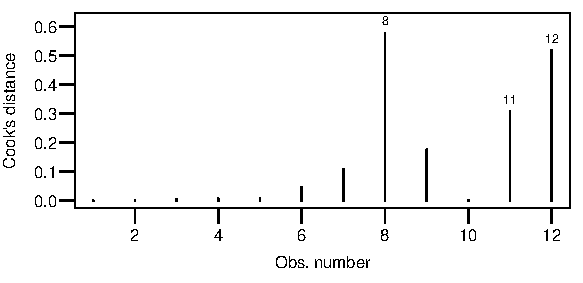
\includegraphics[scale = 0.8]{figure/RC-H13-022c}
\end{figure}

We see that Observations 8 and 12 exceed our 0.4 threshold. However, this has to be interpretted with caution. Unlike the normal linear regression, in a Poisson regression the observations with higher values of $\mu$ are expected to have higher influence than those with lower values of $\mu$.
\end{frame}



%%%%%%%%%%%%%%%%%%%%%%%%%%%%%%%%%%%%%%%%%%%%%%%%%%%%%%%%%%%%%%%%%%%%%%%%%%%%%%%%%%%%%%%%%%%
\BeginSection{Interpretting the GLM output}
%%%%%%%%%%%%%%%%%%%%%%%%%%%%%%%%%%%%%%%%%%%%%%%%%%%%%%%%%%%%%%%%%%%%%%%%%%%%%%%%%%%%%%%%%%%


\begin{frame}[fragile]
\frametitle{Submissions to CRAN using Poisson regression\ldots}
\framesubtitle{Inference}
Let's look at the estimated rate of annual increase in submissions of R packages to the CRAN.
\bigskip

Recall that our model for the expected number of submissions to the CRAN is 
\[ \mu = \exp(\beta_0+\beta_1 \times Year) = \exp(\beta_0) \times \exp(\beta_1)^{Year} \] 
so we need to exponentiate our estimate and its confidence interval.
\bigskip

The annual multiplicative effect on $\mu$ is $\exp(\beta_1)$, and our estimated value of this effect is  $\exp(\hat{\beta}_1)$:
\begin{knitrout}\scriptsize
\definecolor{shadecolor}{rgb}{0.969, 0.969, 0.969}\color{fgcolor}\begin{kframe}
\begin{alltt}
\hlstd{> }\hlcom{## The estimated annual multiplier}
\hlstd{> }\hlkwd{exp}\hlstd{(CRAN.quasigfit}\hlopt{$}\hlstd{coef[}\hlstr{"Year"}\hlstd{])}
\end{alltt}
\begin{verbatim}
    Year 
1.896614 
\end{verbatim}
\end{kframe}
\end{knitrout}

\end{frame}


\begin{frame}[fragile]
\frametitle{Submissions to CRAN using Poisson regression\ldots}
\framesubtitle{Confidence intervals for effects}

We can still use the function \rcode{confint()} to get confidence intervals for the parameters.  
\medskip

\begin{knitrout}\scriptsize
\definecolor{shadecolor}{rgb}{0.969, 0.969, 0.969}\color{fgcolor}\begin{kframe}
\begin{alltt}
\hlstd{> }\hlkwd{exp}\hlstd{(}\hlkwd{confint}\hlstd{(CRAN.quasigfit))}
\end{alltt}


{\ttfamily\noindent\itshape\color{messagecolor}{Waiting for profiling to be done...}}\begin{verbatim}
               2.5 %   97.5 %
(Intercept) 0.000000 0.000000
Year        1.745819 2.075781
\end{verbatim}
\end{kframe}
\end{knitrout}

\bigskip

Sometimes you might see \rcode{confint.default()} used instead.

\begin{knitrout}\scriptsize
\definecolor{shadecolor}{rgb}{0.969, 0.969, 0.969}\color{fgcolor}\begin{kframe}
\begin{alltt}
\hlstd{> }\hlkwd{exp}\hlstd{(}\hlkwd{confint.default}\hlstd{(CRAN.quasigfit))}
\end{alltt}
\begin{verbatim}
               2.5 %   97.5 %
(Intercept) 0.000000 0.000000
Year        1.739517 2.067898
\end{verbatim}
\end{kframe}
\end{knitrout}

They are doing slightly different things, based on two different approximations. In most cases they give very similar results.
\bigskip

It is generally best to use \rcode{confint()} rather than \rcode{confint.default()}. See STATS 730 for the reason why.

\end{frame}



\begin{frame}[fragile]
\frametitle{Submissions to CRAN using Poisson regression\ldots}
\framesubtitle{Confidence intervals for effects\ldots}

So, our Executive Summary would say that the expected annual number of submissions to CRAN multiplies by between 1.75 and 2.08 times each year.
That is, it increases by between 75\% and 108\% per year.

\medskip\medskip

[This compares to a median multiplier of between 2.00 and 2.40 times each year from the naive \rcode{lm} fit to $\log(y).$]

\medskip\medskip

{\large Note that the GLM model is making statements about the {\bf mean} rather than the {\bf median}. This is because the GLM does not transform $y$.}
\end{frame}


\begin{frame}[fragile]
\frametitle{Submissions to CRAN using Poisson regression\ldots}
\framesubtitle{Confidence interval for expected number of submissions}

And finally, we will use the quasi-Poisson model to estimate the expected number of submissions in 2017. 
We first calculate the confidence interval on the linear predictor scale, and then exponentiate.

\begin{knitrout}\scriptsize
\definecolor{shadecolor}{rgb}{0.969, 0.969, 0.969}\color{fgcolor}\begin{kframe}
\begin{alltt}
\hlstd{> }\hlstd{pred2017.quasi}\hlkwb{=}\hlkwd{predict}\hlstd{(CRAN.quasigfit, predCRAN.df,} \hlkwc{se.fit}\hlstd{=}\hlnum{TRUE}\hlstd{)}
\hlstd{> }\hlcom{# CI for log mean}
\hlstd{> }\hlstd{lower} \hlkwb{=} \hlstd{pred2017.quasi}\hlopt{$}\hlstd{fit}\hlopt{-}\hlnum{1.96}\hlopt{*}\hlstd{pred2017.quasi}\hlopt{$}\hlstd{se.fit}
\hlstd{> }\hlstd{upper} \hlkwb{=} \hlstd{pred2017.quasi}\hlopt{$}\hlstd{fit}\hlopt{+}\hlnum{1.96}\hlopt{*}\hlstd{pred2017.quasi}\hlopt{$}\hlstd{se.fit}
\hlstd{> }\hlcom{#CI for mean value}
\hlstd{> }\hlstd{pred2017.ci.mean}\hlkwb{=}\hlkwd{exp}\hlstd{(}\hlkwd{c}\hlstd{(lower, upper))}
\hlstd{> }\hlstd{pred2017.ci.mean}
\end{alltt}
\begin{verbatim}
        1         1 
 6626.596 10383.014 
\end{verbatim}
\end{kframe}
\end{knitrout}
\medskip

So our Executive Summary would say that the expected number of submissions to CRAN in 2017 is between 6600 and 10400.

\medskip

This compares to the estimated median number being between 6600 and 25100 from the naive \rcode{lm} fit to $\log(y)$.

\end{frame}


\begin{frame}[fragile]
\frametitle{Submissions to CRAN using Poisson regression\ldots}
\framesubtitle{Confidence interval for expected number of submissions...}

The above calculations are done for us using the \rcode{predictGLM} function.
\bigskip

The confidence interval on the linear predictor scale is

\begin{knitrout}\scriptsize
\definecolor{shadecolor}{rgb}{0.969, 0.969, 0.969}\color{fgcolor}\begin{kframe}
\begin{alltt}
\hlstd{> }\hlkwd{predictGLM}\hlstd{(CRAN.quasigfit, predCRAN.df)}
\end{alltt}


{\ttfamily\noindent\itshape\color{messagecolor}{***Estimates and CIs are on the link scale***}}\begin{verbatim}
       fit      lwr      upr
1 9.023387 8.798851 9.247922
\end{verbatim}
\end{kframe}
\end{knitrout}

and on the scale of the response variable is

\begin{knitrout}\scriptsize
\definecolor{shadecolor}{rgb}{0.969, 0.969, 0.969}\color{fgcolor}\begin{kframe}
\begin{alltt}
\hlstd{> }\hlkwd{predictGLM}\hlstd{(CRAN.quasigfit, predCRAN.df,}\hlkwc{type}\hlstd{=}\hlstr{"response"}\hlstd{)}
\end{alltt}


{\ttfamily\noindent\itshape\color{messagecolor}{***Estimates and CIs are on the response scale***}}\begin{verbatim}
      fit      lwr      upr
1 8294.82 6626.623 10382.97
\end{verbatim}
\end{kframe}
\end{knitrout}
\bigskip \bigskip
{\bf NOTE:} For GLMs, it is not straightforward to obtain prediction intervals for new values of the response. This is left to STATS 330.
\end{frame}



%%%%%%%%%%%%%%%%%%%%%%%%%%%%%%%%%%%%%%%%%%%%%%%%%%%%%%%%%%%%%%%%%%%%%%%%%%%%%%%%%%%%%%%%%%%
\BeginSection{Closing Remarks}
%%%%%%%%%%%%%%%%%%%%%%%%%%%%%%%%%%%%%%%%%%%%%%%%%%%%%%%%%%%%%%%%%%%%%%%%%%%%%%%%%%%%%%%%%%%


\begin{frame}
\frametitle{Linear vs generalized linear model}
The linear model that we fitted to the logged CRAN data on slide \pageref{pg:CRAN LM} has some undesirable properties. 
\bigskip

\begin{itemize}
  \item Logged count data do not have equal variance.\footnote{In fact, if $Y$ is Poisson, then $\Var(\log(Y))=\infty$!!!}
  \item Logged count data are highly variable for small expected counts.
  \item Logged count data can not handle a zero count, since $\log(0)$ is negative infinity.
\end{itemize}
\bigskip

The influence plot from the LM fitted to the logged CRAN data showed that the 2nd and 3rd observations were the most influential. This is very dangerous, as these are the most unreliable data points. 
 
\end{frame}


\begin{frame}
\frametitle{Linear vs generalized linear model}
A \rcode{GLM} is a more natural way to model count data. 
\begin{itemize}
  \item It does not transform $y$.
  \item Inference is about {\bf means} (rather than medians).
  \item It accounts for the fact that the variance of $Y$ increases with the mean.
  \item It implicitly allows the higher counts to have more influence.\footnote{This is because the coefficient of variation, CV, is greater for the smaller counts (the CV is the noise-to-signal ratio, $\sd(Y)/\E[Y]=\frac{1}{\sqrt{\mu}}$).}
\end{itemize}
\bigskip

The GLM better models the CRAN data:
\begin{itemize}
  \item The plot of fitted values versus residuals clearly shows the sudden increase at year 8.
  \item The influence plot better shows the true influence of each observation.
  \item It results in narrower confidence intervals for the expected annual increase and expected future counts.
\end{itemize}
\bigskip

\end{frame}


\begin{frame}
\frametitle{Linear vs generalized linear model}
The two key points of difference are:
\medskip

\begin{itemize}
\item $Y|x$ is assumed to be a Poisson distributed count variable (rather than a
normally distributed continuous variable).

\item
Instead of our model being of additive form
\[ \E[Y|x] = {\beta_0 +  \beta_1 x + \dots} \]
it is of multiplicative form
\[ \E[Y|x] = \exp(\beta_0 +  \beta_1 x + \dots) \]
or equivalently
\[ \log (\E[Y|x]) = \beta_0 +  \beta_1 x + \dots \]
\end{itemize}
\bigskip

% Here, ``linear model'' might be $\beta_0 +  \beta_1 x$, say 
% (in the case of a simple linear regression with explanatory variable $x$)
{\bf NOTE:} The GLM transforms the linear model rather than transforming $Y$.
\end{frame}



\begin{frame}
\frametitle{Linear on log scale vs generalized linear model}
In Chapter 6 we logged our response variable before fitting the linear model.
This assumes that the logged reponses are normally distributed and that

\[ \E[\log(Y|x)] = \beta_0 +  \beta_1 x + \dots \]

We saw that, under the above model 
\[ \E[Y|x] \ne \exp(\beta_0 +  \beta_1 x + \dots)\]
and that was why we had to make inference about population medians.
\bigskip \bigskip

In comparison, in the GLM the order of $\log$ and $\E$ is reversed
\[ \log (\E[Y|x]) = \beta_0 +  \beta_1 x + \dots \]

\end{frame}

%%%%%%%%%%%%%%%%%%%%%%%%%%%%%%%%%%%%%%%%%%%%%%%%%%%%%%%%%%%%%%%%%%%%%%%%%%%%%%%%%%%%%%%%%%%
\BeginSection{Relevant \rcode{R}-code}
%%%%%%%%%%%%%%%%%%%%%%%%%%%%%%%%%%%%%%%%%%%%%%%%%%%%%%%%%%%%%%%%%%%%%%%%%%%%%%%%%%%%%%%%%%%



\begin{frame}[fragile]
\frametitle{Most of the \rcode{R}-code you need for this chapter}
We started by identifying what our response is -- in this case a count. Therefore our response data is definitely not from a normal distribution. As $Y$ is a count variable we propose to model it using the Poisson distribution.
\bigskip

Instead of using \rcode{lm} we use \rcode{glm}, and add \rcode{family=poisson}.

\begin{knitrout}\scriptsize
\definecolor{shadecolor}{rgb}{0.969, 0.969, 0.969}\color{fgcolor}\begin{kframe}
\begin{alltt}
\hlstd{> }\hlstd{CRAN.gfit}\hlkwb{=} \hlkwd{glm}\hlstd{(Number}\hlopt{~}\hlstd{Year,}\hlkwc{family}\hlstd{=poisson,}\hlkwc{data}\hlstd{=CRAN.df)}
\hlstd{> }\hlkwd{summary}\hlstd{(CRAN.gfit)}
\end{alltt}
\end{kframe}
\end{knitrout}

Look at  fitted vs residual plot and make sure there's no trend you've missed and/or atypical observations.

\begin{knitrout}\scriptsize
\definecolor{shadecolor}{rgb}{0.969, 0.969, 0.969}\color{fgcolor}\begin{kframe}
\begin{alltt}
\hlstd{> }\hlkwd{plot}\hlstd{(CRAN.gfit,} \hlkwc{which} \hlstd{=} \hlnum{1}\hlstd{)}
\end{alltt}
\end{kframe}
\end{knitrout}

Do {\bf NOT} check for normality!

Influence can still be assessed using \rcode{cooks20x}, but be aware that larger counts will naturally tend to be more influential than smaller counts.
\end{frame}



\begin{frame}[fragile]
\frametitle{Most of the \rcode{R}-code you need for this chapter...}

To check if the data are consistent with the Poisson model you use

\begin{knitrout}\scriptsize
\definecolor{shadecolor}{rgb}{0.969, 0.969, 0.969}\color{fgcolor}\begin{kframe}
\begin{alltt}
\hlstd{> }\hlnum{1} \hlopt{-} \hlkwd{pchisq}\hlstd{(CRAN.gfit}\hlopt{$}\hlstd{deviance,CRAN.gfit}\hlopt{$}\hlstd{df.residual)}
\end{alltt}
\end{kframe}
\end{knitrout}

and if the \pval{} is very small (i.e., less that 0.05) then you can to deal with this 
using the quasi-Poisson model: 

\begin{knitrout}\scriptsize
\definecolor{shadecolor}{rgb}{0.969, 0.969, 0.969}\color{fgcolor}\begin{kframe}
\begin{alltt}
\hlstd{> }\hlstd{CRAN.quasigfit} \hlkwb{=} \hlkwd{glm}\hlstd{(Number} \hlopt{~} \hlstd{Year,} \hlkwc{family} \hlstd{= quasipoisson,} \hlkwc{data} \hlstd{= CRAN.df)}
\end{alltt}
\end{kframe}
\end{knitrout}
\medskip

Once you've chosen your final model you can interpret the effect of the variables as a 
multiplicative change in the {\bf mean} or expected value:
\begin{knitrout}\scriptsize
\definecolor{shadecolor}{rgb}{0.969, 0.969, 0.969}\color{fgcolor}\begin{kframe}
\begin{alltt}
\hlstd{> }\hlkwd{exp}\hlstd{(}\hlkwd{confint}\hlstd{(CRAN.quasigfit))}
\end{alltt}
\end{kframe}
\end{knitrout}

If you wish to estimate a 95\% CI for an expected value 
use \rcode{predictGLM}, or do it the hard way as follows:

\begin{knitrout}\scriptsize
\definecolor{shadecolor}{rgb}{0.969, 0.969, 0.969}\color{fgcolor}\begin{kframe}
\begin{alltt}
\hlstd{> }\hlstd{pred2017.quasi}\hlkwb{=}\hlkwd{predict}\hlstd{(CRAN.quasigfit, predCRAN.df,}\hlkwc{se.fit}\hlstd{=}\hlnum{TRUE}\hlstd{)}
\hlstd{> }\hlcom{# CI for log mean}
\hlstd{> }\hlstd{lower} \hlkwb{=} \hlstd{pred2017.quasi}\hlopt{$}\hlstd{fit}\hlopt{-}\hlnum{1.96}\hlopt{*}\hlstd{pred2017.quasi}\hlopt{$}\hlstd{se.fit}
\hlstd{> }\hlstd{upper} \hlkwb{=} \hlstd{pred2017.quasi}\hlopt{$}\hlstd{fit}\hlopt{+}\hlnum{1.96}\hlopt{*}\hlstd{pred2017.quasi}\hlopt{$}\hlstd{se.fit}
\hlstd{> }\hlcom{#CI for mean value}
\hlstd{> }\hlstd{pred2017.ci.mean}\hlkwb{=}\hlkwd{exp}\hlstd{(}\hlkwd{c}\hlstd{(lower, upper))}
\hlstd{> }\hlstd{pred2017.ci.mean}
\end{alltt}
\end{kframe}
\end{knitrout}

\end{frame}

\end{document}
